% Visualisasi metode cosine dari dosen (rapat 13 Nov 2026, menit 07:03-10:00; papan tulis Paint).
% Kompilasi (dari folder ini): pdflatex cosine_dosen.tex && pdftoppm -png -r 300 -singlefile cosine_dosen.pdf cosine_dosen
\documentclass[border=6pt]{standalone}
\usepackage{amssymb}
\usepackage{mathptmx}
\usepackage{tikz}
\usetikzlibrary{arrows.meta, shadows, calc, positioning}

\definecolor{ink}{HTML}{3A3936}
\definecolor{muted}{HTML}{8A8984}
\definecolor{dataF}{HTML}{F0EFEC}
\definecolor{modelE}{HTML}{2A78D6}\definecolor{modelF}{HTML}{DCE9F9}
\definecolor{augE}{HTML}{EB6834}\definecolor{augF}{HTML}{FDE3D6}
\definecolor{opE}{HTML}{6250D6}\definecolor{opF}{HTML}{EBE9FB}
\definecolor{lossE}{HTML}{1BAF7A}\definecolor{lossF}{HTML}{D9F3E9}

\tikzset{
  every node/.style={font=\small, text=ink, align=center},
  base/.style={rectangle, rounded corners=3pt, minimum height=12mm, inner sep=3pt, line width=0.8pt},
  data/.style={base, fill=dataF, draw=muted, text width=18mm},
  model/.style={base, fill=modelF, draw=modelE, text width=18mm},
  weak/.style={base, fill=modelF, draw=modelE, line width=1.3pt, text width=38mm},
  strong/.style={base, fill=augF, draw=augE, line width=1.3pt, text width=38mm},
  stp/.style={base, fill=white, draw=muted, text width=38mm},
  tensor/.style={rectangle, fill=white, draw=ink, line width=0.8pt, minimum width=6mm, minimum height=9mm,
                 double copy shadow={shadow xshift=1.6pt, shadow yshift=1.6pt, draw=ink, fill=white}},
  flow/.style={-{Stealth[length=2.3mm]}, line width=0.8pt, draw=ink, rounded corners=4pt},
  title/.style={font=\small\bfseries, anchor=west},
  note/.style={font=\footnotesize\itshape, text=muted},
}
\newcommand{\sub}{\footnotesize\color{muted}}

\begin{document}
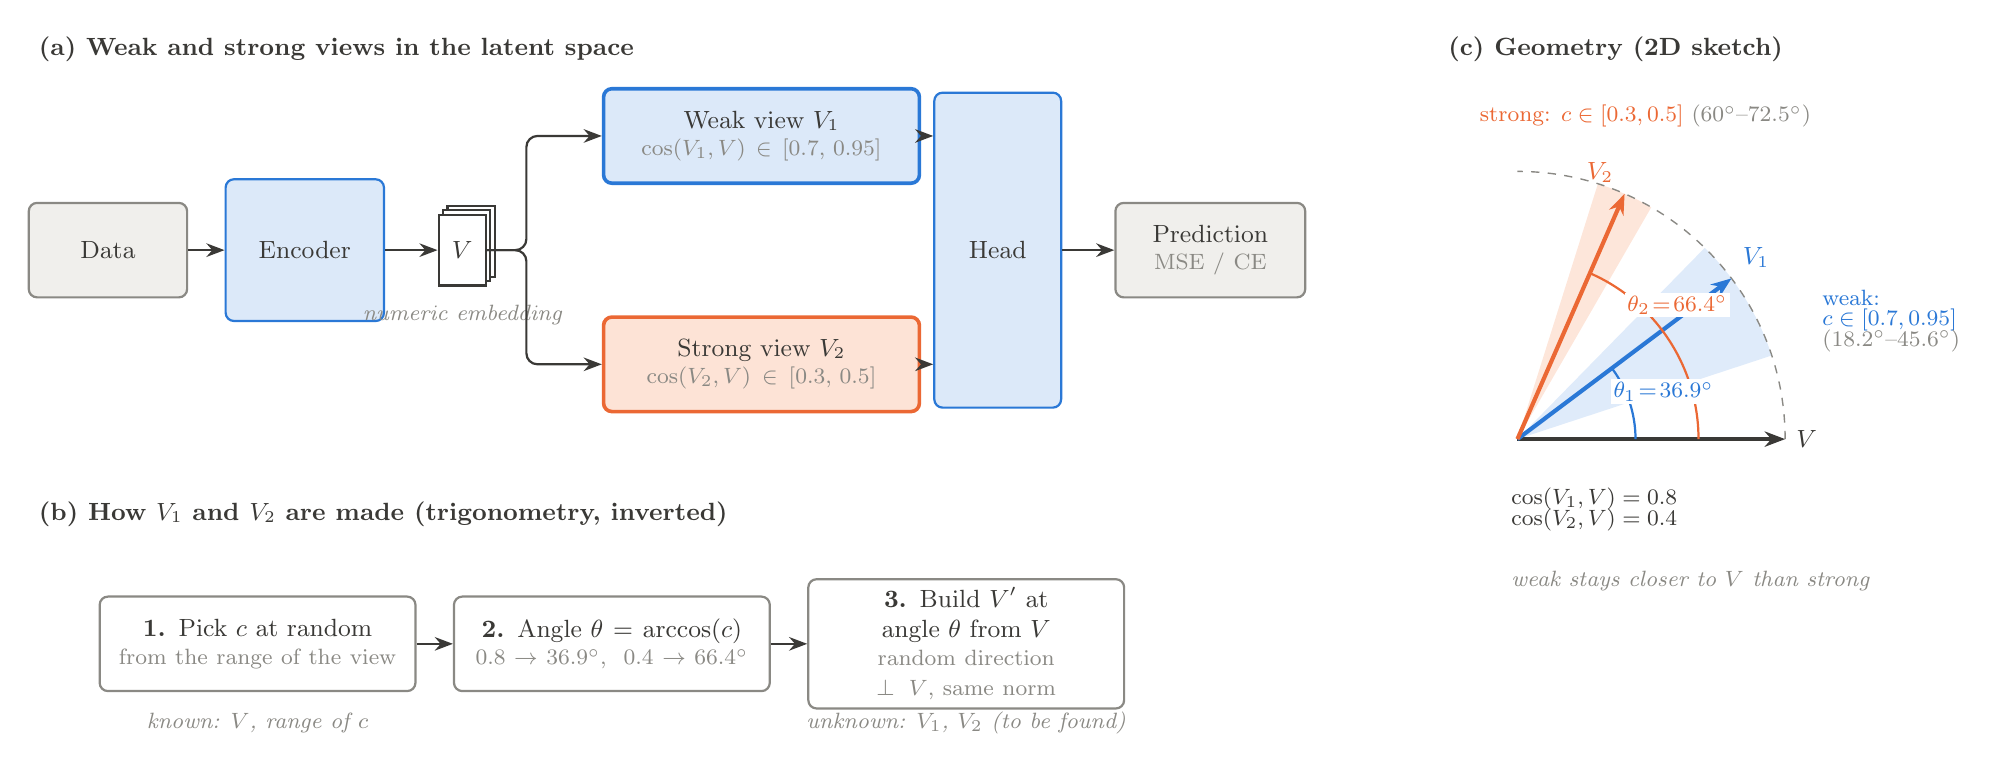
\begin{tikzpicture}

% ================= (a) alur =================
\node[title] at (-1.0, 2.55) {(a) Weak and strong views in the latent space};

\node[data]  (data) at (0,0) {Data};
\node[model, minimum height=18mm] (enc) at (2.5,0) {Encoder};
\node[tensor] (v) at (4.5,0) {$V$};
\node[note, below=3pt of v] {numeric embedding};

\node[weak]   (w) at (8.3, 1.45) {Weak view $V_1$\\[-1pt]{\sub $\cos(V_1, V)\in[0.7,\,0.95]$}};
\node[strong] (s) at (8.3,-1.45) {Strong view $V_2$\\[-1pt]{\sub $\cos(V_2, V)\in[0.3,\,0.5]$}};
\node[model, minimum height=40mm, text width=14mm] (head) at (11.3,0) {Head};
\node[data, text width=22mm] (out) at (14.0,0) {Prediction\\[-1pt]{\sub MSE / CE}};

\draw[flow] (data) -- (enc);
\draw[flow] (enc) -- (v);
\draw[flow] (v.east) -- ++(0.5,0) |- (w.west);
\draw[flow] (v.east) -- ++(0.5,0) |- (s.west);
\draw[flow] (w) -- (w -| head.west);
\draw[flow] (s) -- (s -| head.west);
\draw[flow] (head) -- (out);

% ================= (b) langkah =================
\node[title] at (-1.0,-3.35) {(b) How $V_1$ and $V_2$ are made (trigonometry, inverted)};

\node[stp] (s1) at (1.9,-5.0)  {\textbf{1.} Pick $c$ at random\\[-1pt]{\sub from the range of the view}};
\node[stp] (s2) at (6.4,-5.0)  {\textbf{2.} Angle $\theta=\arccos(c)$\\[-1pt]{\sub 0.8 $\to$ 36.9$^\circ$, \ 0.4 $\to$ 66.4$^\circ$}};
\node[stp] (s3) at (10.9,-5.0) {\textbf{3.} Build $V'$ at angle $\theta$ from $V$\\[-1pt]{\sub random direction $\perp V$, same norm}};
\draw[flow] (s1) -- (s2);
\draw[flow] (s2) -- (s3);
\node[note] at (1.9,-6.0) {known: $V$, range of $c$};
\node[note] at (10.9,-6.0) {unknown: $V_1$, $V_2$ (to be found)};

% ================= (c) geometri =================
\begin{scope}[shift={(17.9,-2.4)}]
  \node[title] at (-1.0,4.95) {(c) Geometry (2D sketch)};
  \def\R{3.4}
  % rentang weak (18.2 - 45.6 derajat) dan strong (60 - 72.5 derajat)
  \fill[modelF, opacity=0.9] (0,0) -- (18.2:\R) arc (18.2:45.6:\R) -- cycle;
  \fill[augF,   opacity=0.9] (0,0) -- (60:\R)   arc (60:72.5:\R)   -- cycle;
  \draw[muted, dashed, line width=0.5pt] (0:\R) arc (0:90:\R);
  % vektor
  \draw[-{Stealth[length=2.6mm]}, line width=1.5pt, ink] (0,0) -- (0:\R) node[right, font=\small] {$V$};
  \draw[-{Stealth[length=2.6mm]}, line width=1.5pt, modelE] (0,0) -- (36.9:\R) node[above right, font=\small, text=modelE] {$V_1$};
  \draw[-{Stealth[length=2.6mm]}, line width=1.5pt, augE] (0,0) -- (66.4:\R) node[above left, font=\small, text=augE] {$V_2$};
  % busur sudut
  \draw[modelE, line width=0.8pt] (0:1.5) arc (0:36.9:1.5);
  \draw[augE,   line width=0.8pt] (0:2.3) arc (0:66.4:2.3);
  \node[font=\footnotesize, text=modelE, fill=white, inner sep=1pt] at (18:1.95) {$\theta_1\!=\!36.9^\circ$};
  \node[font=\footnotesize, text=augE,   fill=white, inner sep=1pt] at (40:2.65) {$\theta_2\!=\!66.4^\circ$};
  % keterangan rentang
  \node[font=\footnotesize, text=modelE, anchor=west, align=left] at (3.75,1.5) {weak:\\[-2pt]$c\in[0.7,0.95]$\\[-2pt]{\sub (18.2$^\circ$--45.6$^\circ$)}};
  \node[font=\footnotesize, text=augE, anchor=west] at (-0.6,4.1) {strong: $c\in[0.3,0.5]$ {\sub (60$^\circ$--72.5$^\circ$)}};
  \node[font=\footnotesize, anchor=north west, align=left] at (-0.2,-0.5) {$\cos(V_1,V)=0.8$\\[-2pt]$\cos(V_2,V)=0.4$};
  \node[note, anchor=north west] at (-0.2,-1.55) {weak stays closer to $V$ than strong};
\end{scope}

\end{tikzpicture}
\end{document}
